\section{Frequency and Phase Estimation}%
\label{sec:freq_est}

Frequency and phase estimation, also called carrier synchronization, is the next step after detection for coherent demodulation.
In this section, we discuss the estimation algorithm by assuming the time synchronization of the preamble is perfect, i.e., 
the observation window contains the complete preamble. For the same reason as in the detection section, we first derive the estimator
by assuming the effect of fractional delay $\Delta p$ is neglected.
Later in simulation section, we will show how much the value of fractional delay degrades the estimating accuracy of estimators by
comparing with different sampling rate.
% I forget to say in last meeting, the plot was truly obtained from a random sequence but with a good autocorrelation property.
% For this time, I compared with the reason with my previous sequence and gold sequence, the result shows the same.
% For figure 2, I think at 0 dB, since the SD estimator may not be accurate enough, the generalized correlation may not tend to be perfectly uncorrelated.
% For this reason, I just keep the previous results with some other modifications for this time.

For estimating frequency offset $\delta$ and the phasor $S=Ae^{j\phi}$, the maximum likelihood (ML) estimation of the parameters in~\eqref{eq:model} is given by

\begin{equation}
\label{eq:ML_f_S}
  \hat{\delta},\hat{S}=\min_{\delta,S=Ae^{j\phi}}\sum_{n=0}^{N-1}|r_n-s_nSe^{j2\pi\delta n}|^{2}.
\end{equation}
% extension to reviewer 1, comment 3
By taking the Wirtinger derivative with respect to $S$ and setting it equal to zero, a 
closed form for the estimated phasor $\hat{S}$ is readily derived,

\begin{equation}
    \label{eq:opt_S}
    \hat{S}=\frac{\sum_{n=0}^{N-1}{r_{n}s_n^{*}e^{-j2\pi\hat{\delta} n}}}{\sum_{n=0}^{N-1}|s_{n}|^2},
  \end{equation}
and $\hat{\phi}=\arg\{S\}$. It can be seen the estimate of phasor $\hat{S}$ relies on the estimate of frequency $\hat{\delta}$.
Thus, the frequency and phasor offset estimates are
joint estimates. Moreover, by plugging~\eqref{eq:opt_S} into~\eqref{eq:generalized_corr}, 
changing from taking the real value by absolute value, an approximate GLRT based detector finally reduces to

\begin{equation}
  \label{eq:reduced_GLRT_detector}
  \rho(p) \approx
  \frac{|\tilde{S}_p|}
  {||\bm{r}_{p}||\cdot||\bm{s}||} \LRT{H_1}{H_0} \gamma
\end{equation}
where $\tilde{S}$ denotes the frequency-corrected cross-correlation (the numerator)
of phasor estimate in~\eqref{eq:opt_S}, and $||\bm{s}||$ is the Euclidean norm of the preamble. 
Note, compared with~\eqref{eq:generalized_corr},
\eqref{eq:reduced_GLRT_detector} greatly lowers the computational complexity of the detector.

% extension to reviewer 1, comment 3, reviewer 3, comment 4
The frequency estimate is obtained similarly as the zero of the
derivative of~\eqref{eq:ML_f_S},

\begin{equation}
    \label{eq:intm_neces_cond1}
    \sum_{n=0}^{N-1}{(r_{n}s_n^{*}S^{*}ne^{-j2\pi \delta n}-s_ns_n^{*}n)=0}.
    \end{equation}
Note $\sum_{n=0}^{N-1}{s_ns_n^{*}n}$ is real
valued, which results in the imaginary part of left hand side of~\eqref{eq:intm_neces_cond1} be zero;
By plugging the estimate $\hat{S}$ of~\eqref{eq:opt_S} into~\eqref{eq:intm_neces_cond1} and rearranging the order of indexes, yields

\begin{equation}
    \label{eq:intm_neces_cond2}
    \Im\bigg\{\sum_{m=0}^{N-1}{\sum_{n=0}^{N-1}{nr_{n}r_{m}^{*}s_n^{*}s_me^{j2\pi \delta(m-n)}}}\bigg\} = 0.
  \end{equation}
A change of variables let us focus on the difference between sampling instances $m$ and $n$.
Defining $k{=}m-n$,~\eqref{eq:intm_neces_cond2} becomes

\begin{equation}
    \label{eq:intm_neces_cond3}
    \Im\bigg\{\sum_{m=0}^{N-1}{\sum_{k{=}m-(N-1)}^{m}{(m{-}k)r_{m-k}r_{m}^{*}s_{m-k}^{*}s_me^{j2\pi \delta k}}}\bigg\}=0.
  \end{equation}
Reversing the order of summation in~\eqref{eq:intm_neces_cond3}, we get

\begin{equation}
    \begin{aligned}
    \label{eq:intm_neces_cond4}
    \Im\bigg\{&\sum_{k=-(N-1)}^{0}\sum_{m=0}^{N-1+k}{(m{-}k)r_{m-k}r_{m}^{*}s_{m-k}^{*}s_me^{j2\pi \delta k}+}\\
    &\quad~~~~~~~~~~~~~~\sum_{k=1}^{N-1}\sum_{m=k}^{N-1}{(m{-}k)r_{m-k}r_{m}^{*}s_{m-k}^{*}s_me^{j2\pi \delta k}}\bigg\}= 0.
    \end{aligned}
  \end{equation}
Note, the term for $k{=}0$ in~\eqref{eq:intm_neces_cond4} can be eliminated since it is real-valued. For $k \neq 0$, the positive and negative indices $k$ are symmetric. 
After grouping terms appropriately, the necessary condition for $\hat{\delta}$ is given by

\begin{equation}
    \label{eq:delta}
    J(\hat{\delta}) = \Im\bigg\{\sum_{k=1}^{N-1}{\sum_{m=k}^{N-1}{kr_{m-k}r_m^{*}s_{m-k}^{*}s_m}e^{j2\pi\hat{\delta}k}}\bigg\}=0.
    \end{equation}
This expression is fundamentally equivalent to conditions provided by Luise and Reggiannini~\cite{Luise_Reggiannini_95} and Fitz~\cite{Fitz_94}.
However,~\eqref{eq:delta} explicitly allows for pulse shaping and oversampling.
Note, the estimator $\hat{\delta}$ in~\eqref{eq:delta} has no closed-form
solution.
In~\cite{Luise_Reggiannini_95}, it is approximated by replacing the exponential with its
Taylor series expansion.
In~\cite{Fitz_94}, an approximate solution is obtained via Euler's
identity for large $N$.
Both solutions have computational complexity $O(N^2)$ reflecting the
double summation.

Since our paper focus on the joint detection and estimation problem, we propose a family of alternative solutions to~\eqref{eq:delta}.
A coarse solution with $O(N)$ complexity is used for operating at high sampling
rate during the sequential GLRT detection;
It prioritizes the low complexity at the expense of some loss of accuracy. 
A fine solution is used to improve the estimation accuracy 
for the coherent demodulation once the preamble has been detected.
The two solutions are illustrated with details in the next sections.

\subsection{Solution I: (Coarse) Single-Difference (SD) Estimator}

The first estimator is rooted in the insight that at high SNR environment, every lag $k$ in~\eqref{eq:delta} can be used to
approximate the true frequency offset $\bar{\delta}$. Assume noise is small, i.e.,
$r_m \approx s_mAe^{j(2\pi \bar{\delta} m+\phi)}$,~\eqref{eq:delta} can be expanded to

\begin{equation}
    \label{eq:delta_extens_no_noise}
    \Im\bigg\{A^2\sum_{k=1}^{N-1}\sum_{m=k}^{N-1}k|s_{m-k}|^2|s_m|^2e^{j2\pi (\hat{\delta}-\bar{\delta})k}\bigg\}=0.
    \end{equation}
Note that in~\eqref{eq:delta_extens_no_noise} the inner summation is purely real for every lag~$k$ if $\hat{\delta}=\bar{\delta}$.
This suggests that an unbiased estimate of frequency offset $\hat{\delta}$ can be obtained by using only a single lag~$k$
from~\eqref{eq:delta}. The approach lowers the complexity from $O(N^2)$ to $O(N)$ and permits a closed-form solution for $\hat{\delta}$.  
While, the disadvantage of the estimator by using single lag $k$ is its insufficient estimating accuracy since it lacks of the processing gain by outer integrator.
Thus, we name the estimator as the coarse Single-Difference (SD) estimator. We just omit "coarse" for simplicity from now.
Just because of the low complexity and moderate estimating accuracy, 
the SD estimator is used for frequency correction of sequential GLRT detector in~\eqref{eq:generalized_corr}. 

\subsubsection{Closed-form expression} 
For one lag $k$, we first give the expression of the (primary) SD estimator that can be directly obtained by reducing~\eqref{eq:delta_extens_no_noise},
\begin{equation}
    \label{eq:delta_SD}
    \est{\delta}{\text{primary}-\sd}(k)=-\frac{\arg\big\{\sum_{m=k}^{N-1}r_{m-k}r_m^*s_{m-k}^*s_m\big\}}{2\pi k}.
\end{equation}

\subsubsection{Performance of the primary SD estimator}
In low SNR environment, i.e., noise effect cannot be ignored, the argument of numerator, denoted as $W(k)$, in~\eqref{eq:delta_SD} can be extended to 

\begin{equation}
  \label{eq:delta_extens_w_noise}
  \begin{aligned}
    &W(k)=\sum_{m=k}^{N-1}r_{m-k}r_m^*s_{m-k}^*s_m \\
    &~=\sum_{m=k}^{N-1} \Big( A^2|s_{m-k}|^2|s_m|^2e^{-j2\pi \bar{\delta} k} + w_m^* S|s_{m-k}|^2s_m e^{j2\pi \bar{\delta}(m-k)}+\\
    &\quad ~~~~~~~~~~~~~~ w_{m-k}S^*|s_m|^2s_{m-k}^* e^{-j2\pi \bar{\delta} m} + w_{m-k}w_m^*s_{m-k}^*s_m \Big) .
  \end{aligned}
\end{equation}

To interpret~\eqref{eq:delta_extens_w_noise}, recognize that the first term of right hand side is
deterministic and provides the mean of the expression. 
The middle two terms yield a zero-mean, complex Gaussian random variable; While,  
the last term performs another zero-mean random variable with a second kind Bessel distribution. 
Note, the two random variables are uncorrelated.
Moreover, we assume $N{-}k$ is large, by central limit theorem, 
the second kind Bessel random variable is considered approximately Gaussian.      
Thus,~\eqref{eq:delta_extens_w_noise} is summarized as
% ask for more details are lack of. 

\begin{equation}
  \begin{aligned}
    \label{eq:ori_pdf_W}
    W(k) \sim \cn\bigg(\Big(
    \frac{N{-}k}{A^2}\Big){\Big(\frac{E_s}{M}\Big)}^2e^{-j2\pi \bar{\delta} k},
    2&\Big(\frac{N{-}k}{A^4}\Big)\frac{N_0}{2}{\Big(\frac{E_s}{M}\Big)}^3+ \\
    &\Big(\frac{N{-}k}{A^4}\Big)\Big(\frac{N_0}{2}\Big)^2{\Big(\frac{E_s}{M}\Big)}^2\bigg),
  \end{aligned}
\end{equation}
where $A^2|s_m|^2 {\approx} E_s/M$ denotes the average energy per
sample. A quick test for the primary SD estimator with respect to SNR is to look at the ratio of 
(absolute) square of mean to variance of $W(k)$ in~\eqref{eq:ori_pdf_W}, which is denoted as the output SNR,

\begin{equation}
  \begin{aligned}
    \label{eq:SNR_out_primary}
    \text{SNR}_{\text{out\_primary}}=\frac{|\mu_{W(k)}|^2}{\sigma^2_{W(k)}} 
    =&~\frac{N-k}{ 2\cdot\frac{N_0}{2}\Big/\frac{E_s}{M}+\big(\frac{N_0}{2}\big)^2\Big/\big(\frac{E_s}{M}\big)^2} \\
    =&~\frac{N-k}{2/\text{SNR}_{\text{in}}+1/\text{SNR}_{\text{in}}^2}
  \end{aligned}
\end{equation}
where $\mu_{w(k)}$ and $\sigma^2_{W(k)}$ deonte the mean and variance of $W(k)$ provided in~\eqref{eq:ori_pdf_W}, 
and $\text{SNR}_{\text{in}}=\frac{E_s}{M}\big/\frac{N_0}{2}$ is defined as the average input sample energy to noise power spectral density. In~\eqref{eq:SNR_out_primary}, 
$N-k$, which is the size of integrator in~\eqref{eq:delta_extens_w_noise}, exactly provides the processing gain; At relatively high SNR,
the inverse-square input SNR, which is from the variance of second kind Bessel variable, could be neglected; Thus, the estimating accuracy of primary SD estimator
exhibits a linear relationship with high $\text{SNR}_{\text{in}}$. 
At low input SNR, 
the inverse-square SNR dominates and degrades the $\text{SNR}_{\text{out}}$
of $W(k)$ quadratically, which makes the $\text{SNR}_{\text{out}}$ fast approach and then be lower than the minimum requirement that maintains the required accuracy for building detector and later a fine estimator. 

Now, we will derive the distribution of primary SD estimator.
Recall from~\eqref{eq:delta_SD}, the distribution of $\hat{\delta}_{\text{primary}-\text{SD}}(k)$ requires $\arg\{W(k)\}$.
The complete probability density function (pdf) of $\arg\{W(k)\}$ is derived in appendix \ref{AL},
where it also shows that a good approximation, valid for moderate SNR, 
is Gaussian. Specifically 

\begin{equation}
    \label{eq:sol_pdf_W}
    \arg\{W(k)\} \sim \n\bigg(\angle \mu_{W(k)},\frac{\sigma^2_{W(k)}}{|\mu_{W(k)}|^2}\bigg).
  \end{equation}
Thus,~\eqref{eq:sol_pdf_W} proves the variance of primary SD estimator is inverse proportional to $\text{SNR}_{\text{out}}$ in~\eqref{eq:SNR_out_primary}.
By plugging~\eqref{eq:ori_pdf_W} in~\eqref{eq:sol_pdf_W} without adding second Bessel variance term, the primary SD estimator of~\eqref{eq:delta_SD}
is approximately Gaussian distributed at m-oderate SNR with pdf

\begin{equation}
    \label{eq:pdf_delta}
        \est{\delta}{\text{primary}-\sd}(k) \sim \n \bigg(\bar{\delta},\frac{M}{4\pi^2k^2(N{-}k)E_s/N_0}\bigg).
  \end{equation}  
We see that $\hat{\delta}_{\text{primary}-\text{SD}}(k)$ is unbiased. 
Note, the distribution of primary SD estimator in~\eqref{eq:pdf_delta} only exploits a good fit for moderate SNR due to
the constraint of~\eqref{eq:sol_pdf_W}. A rough calc-ulation for distribution 
at low SNR is to simply replace the variance of Gaussian by variance of second kind Bessel
of~\eqref{eq:ori_pdf_W} and plugging in~\eqref{eq:sol_pdf_W}.
The resulting variance, or equavilently, the mean-squared error (MSE) of the primary SD estimator at low SNR, 
compared to high SNR, is increased by $\frac{M}{4E_s/N_0}$.
% For example, when $E_s/N_0=0.3$, i.e., \numb{-5}\dB, with a normal oversampling factor $M=4$,
% the performance of primary SD estimator is approximately degraded by a factor of 3.3.
The solution to mitigating the increased variance of the primary SD estimator at low SNR
is given in the next section.

\subsubsection{Block-$v$ SD estimator}

\begin{figure}[t]
  \centerline{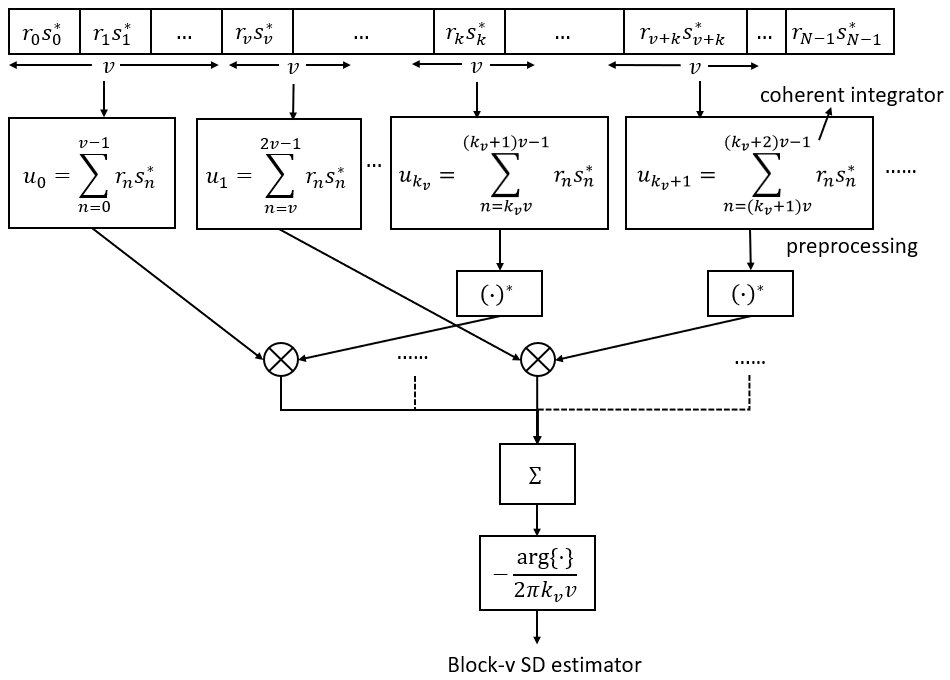
\includegraphics[width=3.4in,height=3.2in]{general_SD_estimator.png}}
  \caption{Flow diagram of implementing the Block-$v$ SD estimator}
  \label{fig:general_SD_estimator}
  \end{figure}

The reason for the primary SD e-stimator of~\eqref{eq:delta_SD} has a relatively bad performance at low SNR is because the large noise
disturbance significantly decorrelates the received signal and the preamble at each sample instant.
An alternative SD estimator is proposed by changing the order of computation in~\eqref{eq:delta_SD}.
Specifically, 
instead of calculating the correlation at each sample instant, 
cross-correlation between $k$ sample instant and then averaging, 
we first average the correlations for some coherent time instants; 
By doing this, some of processing gain is applied to increase the estimating accuracy in every small section of sample instants.
The results are called coherent integrators and the process is called preprocessing.
After that, use the remaining processing gain to integrate 
the coherent integrators between non-coherent time instants.
The details are illustrated in Figure~\ref{fig:general_SD_estimator}. 

In Figure~\ref{fig:general_SD_estimator}, the coherent integrator $u_l$ is formulated by

\begin{equation}
  \label{eq:coherent_integrator}
  u_l=\sum_{n=lv}^{(l+1)v-1}r_ns_n^*, \quad \text{for}~l=0,1,\ldots,N/v{-}1
\end{equation}
where $v$ denotes the number of coherent correlations that are for averaging. 
The value of $v$ is set to be a factor of $N$ to include all sample instants.
$k_v$ denotes the distance between coherent integrators 
that calculates correlation of non-coherent time instants.
Thus, $k_v=\lfloor k/v \rfloor$, where $\lfloor \cdot \rfloor$ represents the floor operation, since $v$ is not necessary to be a factor of $k$.
However, we still assume $k\approx k_vv$ for comparison simplicity. Based on above discussion, the alternative Block-$v$ SD estimator is given by

\begin{equation}
  \label{eq:general_sd_estimator}
  \hat{\delta}_{\text{Block}-v-\text{SD}}(v,k_v)=-\frac{\arg\big\{\sum_{l=k_v}^{N/v-1}u_l^*u_{l-k_v}\big\}}{2\pi k_vv}
\end{equation}
It can be seen that the primary SD estimator in~\eqref{eq:delta_SD} is a special case of Block-$v$ SD estimator when $v=1$.
Thus, we uniformly call the two estimators as the Block-$v$ SD estimator.

Now, we discuss the performance of Block-$v$ SD estimator by focusing on the cross-correlation between the two general coherent integrators in~\eqref{eq:general_sd_estimator}.
Based on~\eqref{eq:coherent_integrator} and the derivation of~\eqref{eq:ori_pdf_W}, the coherent integrator $u_l^*$ is complex Gaussian distributed with probability density function,

\begin{equation*}
  \label{eq:pdf_co_integrator_1}
  u_l^* \sim \cn\bigg(\frac{E_s/MS^*}{A^2}\sum_{n=lv}^{(l+1)v-1}e^{-j2\pi \bar{\delta}n},v\frac{E_s/M}{A^2}\frac{N_0}{2}\bigg),
\end{equation*}
and the pdf of complex Gaussian-distributed $u_{l-k_v}$ is also given by

\begin{equation*}
  \label{eq:pdf_co_integrator_2}
  u_{l-k_v} \sim \cn\bigg(\frac{E_s/MS}{A^2}\sum_{n=(l-k_v)v}^{(l-k_v+1)v-1}e^{j2\pi \bar{\delta}n},v\frac{E_s/M}{A^2}\frac{N_0}{2}\bigg).
\end{equation*}
Note, $u_l^*$ and $u_{l-k}$ are uncorrelated. Compared with~\eqref{eq:delta_extens_w_noise}, the cross-correlation between two coherent integrates $u_l^*$ and $u_{l-k_v}$ also yields a random variable
with a combination of Gaussian and second kind Bessel function. After some algebra, the mean and variance of $u_l^*u_{l-k_v}$, denoted as $\mu_{C_u}$ and $\sigma^2_{C_u}$, can be simplified by, respectively,

\begin{equation}
  \begin{aligned}
  \label{eq:cross_corr_co_inte}
  \mu_{C_u}&=\frac{(E_s/M)^2}{A^2}\sum_{n=lv}^{(l+1)v-1}e^{-j2\pi \bar{\delta}n}\Bigg(\sum_{m=(l-k)v}^{(l-k+1)v-1}e^{j2\pi \bar{\delta}m}\Bigg) \\
  &=\frac{(E_s/M)^2}{A^2}e^{-j2\pi \bar{\delta}k_vv}\Bigg(\frac{\sin(\pi \bar{\delta}v)}{\sin(\pi \bar{\delta})}\Bigg)^2, \\
  \sigma^2_{C_u}&=v^2\frac{(E_s/M)^2}{A^4}\Big(\frac{N_0}{2}\Big)^2+2v\frac{(E_s/M)^3}{A^4}\frac{N_0}{2}\Bigg(\frac{\sin(\pi \bar{\delta}v)}{\sin(\pi \bar{\delta})}\Bigg)^2,
\end{aligned}
\end{equation}
where $\frac{\sin(\pi \bar{\delta}v)}{\sin(\pi \bar{\delta})}$ is one of the Dirichlet function, which appro-aches the maximum value $v$ at $\bar{\delta}=0$ and the first pair of zero crossings at
$\bar{\delta}=\pm 1/v$. Based on~\eqref{eq:SNR_out_primary} and~\eqref{eq:cross_corr_co_inte}, 
the output SNR of Block-$v$ SD estimator in terms of the input SNR yields

\begin{equation}
  \begin{aligned}
    \label{eq:SNR_out_general}
    &\text{SNR}_{\text{out\_Block}-v}=\frac{|\mu_{C_u}|^2}{\sigma^2_{C_u}} \\
    &~~~=\frac{\frac{(Es/M)^4}{A^4}\Big(\frac{\sin(\pi \bar{\delta}v)}{\sin(\pi \bar{\delta})}\Big)^4(N/v-k_v)^2}
    {\Big[v^2\frac{(E_s/M)^2}{A^4}\Big(\frac{N_0}{2}\Big)^2+2v\frac{(E_s/M)^3}{A^4}\frac{N_0}{2}\Big(\frac{\sin(\pi \bar{\delta}v)}{\sin(\pi \bar{\delta})}\Big)^2\Big](N/v{-}k_v)} \\
    &~~~=\frac{(N/v-k_v)\Big(\frac{\sin(\pi \bar{\delta}v)}{\sin(\pi \bar{\delta})}\Big)^4}
    {\frac{v^2}{\text{SNR}_{\text{in}}^2}+\frac{2v}{\text{SNR}_{\text{in}}}\Big(\frac{\sin(\pi \bar{\delta}v)}{\sin(\pi \bar{\delta})}\Big)^2}.
  \end{aligned}
\end{equation}
Some important observations of $\text{SNR}_{\text{out\_Block}-v}$ from~\eqref{eq:SNR_out_general} can be discussed. 
  First, the $\text{SNR}_{\text{out}}$ depends on the value of $|\bar{\delta}|v$.
We begin to consider the case when $|\bar{\delta}|v\ll1$, i.e., $\frac{\sin(\pi \bar{\delta}v)}{\sin(\pi \bar{\delta})} \approx v$
and $(N/v-k_v)v \approx N-k$.
When the input SNR is moderate, the second term of variance dominates and results the nearly same output SNR as in~\eqref{eq:SNR_out_primary};
While at low SNR, the first term of variance dominates and ideally produces an approximate $v$ times larger output SNR than the primary SD estimator,
whi-ch corresponds to the design intention of block-$v$ ($v \geq 2$) SD estimator.
The selection of $v$ trades off the processing gain at low SNR and incurred large frequency offset.

In practice, $|\bar{\delta}|$ is generally not large,
a reasonable assump-tion is to assume $\bar{\delta}$ is in the range of $[-1/v,1/v]$.
By com-paring~\eqref{eq:SNR_out_primary} and~\eqref{eq:SNR_out_general}, it is easy to get
the Block-$v$ SD estimator produces a positive processing gain at low SNR when $|\bar{\delta}|v$ satisfies
$\frac{\sin(\pi \bar{\delta}v)}{\sin(\pi \bar{\delta})} \in [v^{3/4},v]$;
However, The worst case happens when $|\bar{\delta}|v_{\text{min}}$ even also produces a relative large frequency offset, 
i.e., $v_{\text{min}}=2$ and $\frac{\sin(2\pi \bar{\delta})}{\sin(\pi \bar{\delta})}\in [0,2^{3/4})$; 
The Block-$v$ SD estimator will not improve the performance than the primary SD estimator at low SNRs.

Now, let's measure the distribution of Block-$v$ SD estimator at low SNR.
Assume $|\bar{\delta}|v$ always satisfies $v^{3/4}\leq\frac{\sin(\pi \bar{\delta}v)}{\sin(\pi \bar{\delta})}\leq v$,
and the extra processing gain $v$ at relatively low SNR increases the $\text{SNR}_{\text{out\_Blv}}$ to meet the moderate SNR requirement of~\eqref{eq:sol_pdf_W}.
Thus, by plugging~\eqref{eq:cross_corr_co_inte},~\eqref{eq:sol_pdf_W} into~\eqref{eq:general_sd_estimator}, the block-$v$ SD estimator is distributed approximately Gaussian at relatively low SNR with probability density function

\begin{equation}
  \begin{aligned}
  \label{eq:pdf_general_delta}
      \est{\delta}{\text{Block}-v-\text{SD}}(&v,k_v) \\
      &\sim \n \bigg(\bar{\delta},\frac{M^2v^2}{16\pi^2k^2\Big(\frac{\sin(\pi \bar{\delta}v)}{\sin(\pi \bar{\delta})}\Big)^4(N/v{-}k_v)(E_s/N_0)^2}\bigg).
  \end{aligned}
\end{equation} 
Thus, $\est{\delta}{\text{Block}-v-\text{SD}}$ is also unbiased. Moreover, the lag $k_v$ also affects the variance of Block-$v$ SD estimator. The best choice is to choose
$k_v=\lfloor\frac{2N}{3v}\rfloor$ to minimize the variance. However,
it should be noted that if $k_vv$ is too large, 
the frequency estimate $\est{\delta}{\text{Block}-v-\text{SD}}$ 
may suffer the effect of "alasing" if $2\pi|\bar{\delta}|k_vv>\pi$.
The ambiguity problems are common in frequency estimation. The effective method to solve it is based on the robust Chinese reminder theorem.
% should give some reference.

It should be also compared and emphasized the complexity of block-$v$ ($v\geq 2$) SD estimator
with block-1 SD estimator in sequential detection process. The two estimators have the same
complexity for single detection but large computational-complexity difference in sequential detection.
Note, for block-$v$ ($v\geq 2$) SD estimator, because of preprocessing, each sample in received sequence should
be multiplied by the sample in the preamble at same sample instant; 
This greatly limits the way of computing between two adjacent sequential detection.
However, for block-1 SD estimator in~\eqref{eq:delta_SD}, the more efficient way is to 
calculate the autocorrelations for both received and reference sequence with sample difference $k$ and then multiply.
By doing this method, except for the first received sequence,     
we only need to calculate one more autocorrelation for the incoming sample at each detection.
Since the autocorrelations of samples in the preamble can be pre-computed, the argument of~\eqref{eq:delta_SD}
can be computed by the cross-correlation between 
the autocorrelations of received sequence in a shift register
and autocorrelations of reference samples in a fixed vector. 
Thus, compared with block-$v$, block-1 SD estimator greatly reduces the computational redundancy in sequential detection.

\subsection{Solution II: (Fine) Newton-Method (NM) Estimator}

The (block-$v$) SD estimator emphasizes the low-complexity property and is intended to provide merely sufficiently good carrier synchronization
to enable coherent detection. 
Once the signal has been acquired, the accuracy of the block-$v$ SD estimator can be improved by 
investing additional computations. Since detection events are rare, the computational complexity is of little concern.

The principle is to use the Block-$v$ SD estimator as the starting point for a Newton-type iteration 
aimed at finding a better solution to the necessary condition~\eqref{eq:delta}. 
In principle, multiple iterations are possible to produce successively better approximations to the root of
$\J(\hat{\delta})$ in~\eqref{eq:delta}. Specifically, the iterations are given by

\begin{equation}
    \label{eq:iter_NM_est}
    \est{\delta}{\nm}^{(i+1)}=\est{\delta}{\nm}^{(i)}-
    \frac{\J(\est{\delta}{\nm}^{(i)})}{\J^\prime(\est{\delta}{\nm}^{(i)})}
  \end{equation}
where $\est{\delta}{\nm}^{(0)}~{=}~\est{\delta}{\sd}(k_{\opt})$ is the starting point of the iteration and
$\J^\prime(\cdot)$ denotes the derivative of $\J$ with respect to $\hat{\delta}$. Specifically,

\begin{equation}
    \label{eq:derivative of delta}
    J^\prime(\hat{\delta}) = \Im\bigg\{\sum_{k=1}^{N-1}{\sum_{m=k}^{N-1}{j2\pi k^2r_{m-k}r_m^{*}s_{m-k}^{*}s_m}e^{j2\pi\hat{\delta}k}}\bigg\}.
    \end{equation}
Our simulations indicate that only a single iteration is usually sufficient to achieve very good accuracy.


